\documentclass[conference]{IEEEtran}

\usepackage{epsfig}
\usepackage{fancyvrb}

\DefineVerbatimEnvironment%
  {code}{Verbatim}{numbers=left,numbersep=3pt,frame=lines,%
                   xleftmargin=7pt,fontsize=\footnotesize}




\begin{document}


\title{An OSGi-based Sensor Network for \\ Environmental Monitoring}

\author{\authorblockN{XXX}
\authorblockA{San Francisco State University \\
Computer Science Department \\
1600 Holloway Avenue \\
San Francisco, CA 94132 \\
EMail: XXX@sfsu.edu}}


\maketitle
\begin{abstract}
  Abstract.
\end{abstract}


\section{Introduction}

Environmental monitoring depends on the reliable collection of
measurements from remotely deployed sensors and the rapid transfer of
those measurements to data centers where processing and analysis may
take place. Typically, sensors are deployed in out-of-the-way
locations where physical access is limited and connections for
telemetry are poor or nonexistent.   Maintaining the data stream from
these sensors places demands on human resources, requiring site visits
to service the sensors and to download data stored on internal memory.
Consequently, there is a lag of days to months between the time the
sensors perform the measurements and the time the measurements becomes
available.   Advances in battery life and anti-fouling technology have
extended service cycles for field sensors, with the unwanted result of
further delaying access to monitoring data.  In addition, the
dependence on field site visits to alter of sensor characteristics,
such as sampling rate, prevents adjustment in monitoring strategy in
response to rapidly developing events (e.g. oil spills, harmful algal
blooms).

To address these problems of data collection from remote
sensors, we propose to develop an automated end-to-end system based on
proven technology that provides a means to program and interrogate
sensors at the remote field locations and to transmit collected
measurements over long distances to data collections centers where the
data is rapidly processed, archived, and made available to potential
users in near real-time.


\section{Use Case}

Researchers in the geosciences rely on sensor data collected by highly
specialized sensors such as the Seabird or YSI. These sensors are
usually deployed in remote locations that not only make their
maintenance difficult, but also access to their measurements.
Typically the sensors are autonomous in the sense that they can run
for a certain time on battery power and store the measurement data in
internal memory. Only when the sensors are serviced, the measurement
data they have collected since the last servicing are uploaded to a
portable storage device. From there the data can be uploaded to
server. This manual procedure to retrieve sensor data is not only
error prone, but also results in a serious time lag between the time
the sensor performs the measurement and when it becomes available for
further processing. For many applications it would be beneficial to
have near-realtime access to the sensor measurement. Being able to
access data when they become available on the sensor device also
reduces the maintenance overhead.

Start with some related work. Who else has done an OSGi-based
infrastructure for sensor networks? Kleber: I believe you have a few
references. This section should be a combination of a use case (using
the RTC and their YSI sonde as an example) and a requirements
analysis: requirements such as remote management and monitoring
capabilities, time-delayed communication, etc. In this section should
be no mentioned of DSP or OSGi. Length: 1 page.

\section{DSP}

Should describe the OSGi-based NetBEAMS architecture. Total length of
this section: 2 pages.

\subsection{Data Sensor Framework and Platform}

should include a picture of a standalone DSP showing a DC and a DP
(general description only). Explain difference between DSP Framework
and DSP Platform. This section should give a top-level overview.
Subsequent sub-sections should explain certain features of the DSP in
more detail.

\begin{figure}
\centering
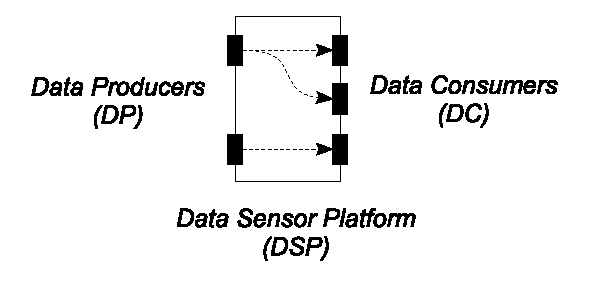
\epsfig{file=dsp, width=7cm}
\caption{\label{FIG_DSP} Data Sensor Platform (DSP).}
\end{figure}

\subsection{DP and DC}

Should give some API sniplets for DP and DC.

\subsection{DSP Message}

Should explain the way DSP Messages are defined: XML Schema and JAXB.

\subsection{Matcher}


\section{NetBEAMS}

Should explain some specific DC and DP we have implemented for
NetBEAMS. Length: 1 - 1.5 pages.

\begin{figure*}
\centering
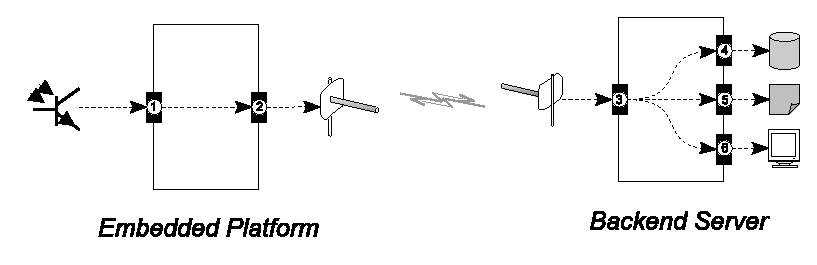
\epsfig{file=netbeams, width=10cm}
\caption{\label{FIG_NETBEAMS} NetBEAMS architecture.}
\end{figure*}

\subsection{YSI Sonde DP}

\subsection{Wire transport DC/DP}

\subsection{Web Managements}


\section{Conclusions and Outlook}

Length (including bibliography): 0.5 pages.

The California coastal region is populated by a vast number of
remotely deployed sensors that monitor environmental conditions
ranging from weather to water quality to ocean surface currents.
These sensors are operated by data providers, including resource
management groups, research scientists, municipalities, and state and
federal agencies, who could use near real-time data streams to inform
decision that impact public health, public safety, and the protection
of resources.  In addition, there are efforts underway at the state
and federal level to collate the data collected by the individual data
providers into integrated monitoring networks that will enhance the
distribution of monitoring data to public, private, and federal users
groups.  Success of these efforts, whether small scale or a large
integrated network, depends on the first step in the data management
process: reliably obtaining data in near real-time from remotely
located sensors.  This step can be the weak link in the data
management pathway when telemetry options are unreliable.  The
availability of a plug-and-play computing platform designed to
communicate with a variety of sensor types and to provide data
telemetry to distant brick and mortar data centers would stabilize
data streams with poor telemetry and allowing expansion of sensor
coverage into regions not presently served.  The low power consumption
and low cost of these units would be particularly beneficial for
applications with long service cycles and for data providers trying to
maintain data streams on a limited budget.

%\bibliography{../literature/lit}
%\bibliographystyle{plain}


\end{document}
